%% LaTeX template for BSc Computing for Games final year project dissertations
%% by Edward Powley
%% Games Academy, Falmouth University, UK

%% Based on:
%% bare_jrnl.tex
%% V1.4b
%% 2015/08/26
%% by Michael Shell
%% see http://www.michaelshell.org/
%% for current contact information.
%%
%% This is a skeleton file demonstrating the use of IEEEtran.cls
%% (requires IEEEtran.cls version 1.8b or later) with an IEEE
%% journal paper.
%%
%% Support sites:
%% http://www.michaelshell.org/tex/ieeetran/
%% http://www.ctan.org/pkg/ieeetran
%% and
%% http://www.ieee.org/

%%*************************************************************************
%% Legal Notice:
%% This code is offered as-is without any warranty either expressed or
%% implied; without even the implied warranty of MERCHANTABILITY or
%% FITNESS FOR A PARTICULAR PURPOSE! 
%% User assumes all risk.
%% In no event shall the IEEE or any contributor to this code be liable for
%% any damages or losses, including, but not limited to, incidental,
%% consequential, or any other damages, resulting from the use or misuse
%% of any information contained here.
%%
%% All comments are the opinions of their respective authors and are not
%% necessarily endorsed by the IEEE.
%%
%% This work is distributed under the LaTeX Project Public License (LPPL)
%% ( http://www.latex-project.org/ ) version 1.3, and may be freely used,
%% distributed and modified. A copy of the LPPL, version 1.3, is included
%% in the base LaTeX documentation of all distributions of LaTeX released
%% 2003/12/01 or later.
%% Retain all contribution notices and credits.
%% ** Modified files should be clearly indicated as such, including  **
%% ** renaming them and changing author support contact information. **
%%*************************************************************************


\documentclass[journal]{IEEEtran}

\usepackage{graphicx}
% Insert additional usepackage commands here
\usepackage{listings}
\usepackage{color}

\definecolor{darkgreen}{rgb}{0, 0.28, 0}

\lstset{language=R,
    basicstyle=\small\ttfamily,
    stringstyle=\color{darkgreen},
    otherkeywords={0,1,2,3,4,5,6,7,8,9},
    morekeywords={TRUE,FALSE},
    deletekeywords={data,frame,length,as,character},
    keywordstyle=\color{blue},
    commentstyle=\color{darkgreen},
}

\begin{document}
%
% paper title
% Titles are generally capitalized except for words such as a, an, and, as,
% at, but, by, for, in, nor, of, on, or, the, to and up, which are usually
% not capitalized unless they are the first or last word of the title.
% Linebreaks \\ can be used within to get better formatting as desired.
% Do not put math or special symbols in the title.
\title{How Does Simulating Human-Like Curiosity Through Exploration Extensions to Agent Behaviour Influence Perception of Smartness in Games?}
%
%
% author name
\author{Tomas Mazurkevic - 1702208}

% The paper headers -- please do not change these, but uncomment one of them as appropriate
% Uncomment this one for COMP320
% \markboth{COMP320: Research Review and Proposal}{COMP320: Research Review and Proposal}
% Uncomment this one for COMP360
\markboth{COMP360: Dissertation}{COMP360: Dissertation}

% make the title area
\maketitle

% As a general rule, do not put math, special symbols or citations
% in the abstract or keywords.
\begin{abstract}
This paper examines the value of exploration extension for simple artificial intelligence behaviour that potentially enhances its perception of smartness. There are many identifiers for \textit{smartness}, however, this will be discussed in the paper with proposed measurements for \textit{smart} AI in todays' games. Due to the nature of this project, curiosity will also be included both in psychological and computational aspects. Moreover, this paper will look into AI importance for games and why it is considered one of the best ways to test real life applications, such as robotics, autonomous driving cars, data mining and much more. The application this paper is proposing could possibly be considered for video game genre walking simulator or robotic in particular. Finally, data will be discussed, providing analysis on whether proposed exploration extension is capable of improving AI's smartness element.
\end{abstract}

\section{Introduction}
% The very first letter is a 2 line initial drop letter followed
% by the rest of the first word in caps.
% 
% form to use if the first word consists of a single letter:
% \IEEEPARstart{A}{demo} file is ....
% 
% form to use if you need the single drop letter followed by
% normal text (unknown if ever used by the IEEE):
% \IEEEPARstart{A}{}demo file is ....
% 
% Some journals put the first two words in caps:
% \IEEEPARstart{T}{his demo} file is ....
% 
% Here we have the typical use of a "T" for an initial drop letter
% and "HIS" in caps to complete the first word.
\IEEEPARstart{T}{hroughout} the last 30 years, researchers have been trying to create clever artificial intelligence (AI) using different methods and algorithms. Recent achievements include AlphaGo being able to beat world champions in Go \cite{alphago} or OpenAI playing Atari games and, in most of them, getting higher scores than human players \cite{mnih2015human}. AI in games, however, is used to create non-player characters (NPCs), which can have very different patterns varying from AI as Adversary to AI as Spectacle \cite{treanor2015ai}. 

AI in video games is crucial when it's used as one of the main mechanics. Intelligent non-player characters (NPCs) are extremely hard to make due to the nature of its complexity. The more complex it is the more outcomes developers will have to consider and the more problems will occur during development \cite{gdchalo2}. Moreover, it tends to use lots of computer resources \cite{gdchalo2}, such as memory, poor run-time, scalability, and others, which brings more challenges.

Some of the very complex algorithms, such as reinforcement learning (RL), deep Q-learning, curiosity-driven, evolution-based and a lot more are being used in video games as testbeds for different disciplines that vary from training algorithms \cite{aiinvideogames}\cite{robotplayground} to robotics \cite{schmidhuber2006developmental}\cite{colledanchise2018behavior}\cite{brady1985artificial}\cite{oudeyer2004intelligent} to Go \cite{schaul2011measuring}\cite{alphago}. However, due to the specificity of games, it is not always the best solution. Depending on the game's design, simple methods or less complex ones can be used instead of previously mentioned algorithms. As an example, Finite State Machine (FSM, Figure \ref{fig:fsm}) became a common one to use after the success of the game F.E.A.R with only using three FSM states \cite{orkin2006three} or Monte Carlo Tree Search (MTCS, Figure \ref{fig:mcts}) \cite{chaslot2008monte}, which has been used in creation of a new paradigm for Go \cite{gelly2011monte}\cite{gelly2012grand}. %288

\begin{figure}
	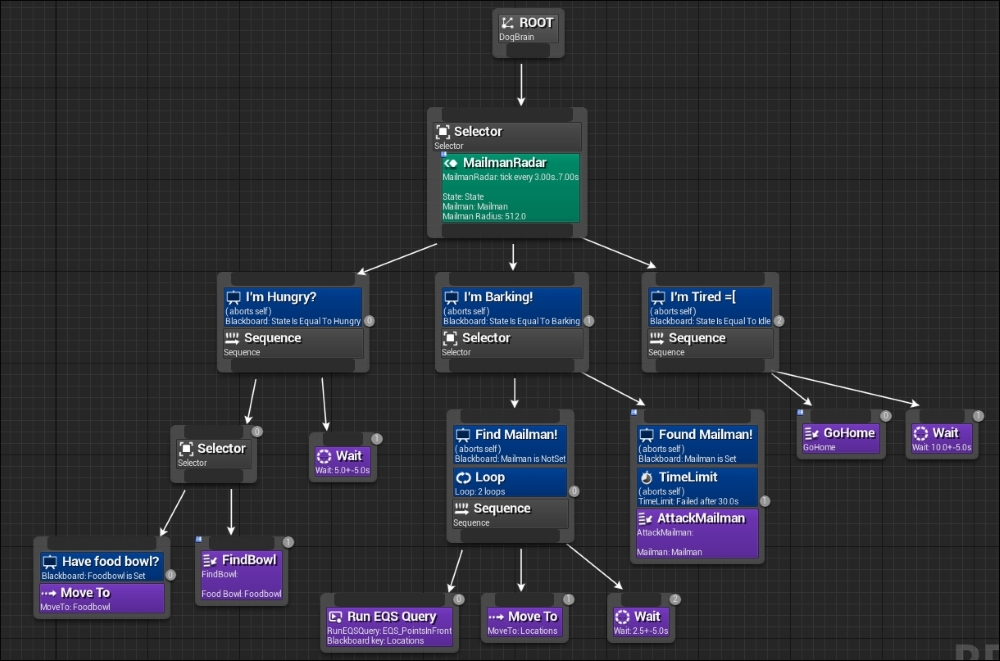
\includegraphics[width=\linewidth]{UnrealBehaviourTree.jpg}
	\caption{Behaviour Tree in Unreal Engine}
	\label{fig:ubt}
\end{figure}

A more simple yet very effective technique for AI creation is behaviour tree (BT). It has first been introduced by Isla \cite{gdchalo2} in videogames such as Halo and is now commonly integrated into game engines like Unreal Engine\footnote{\label{engine}Unreal Engine 4: https://www.unrealengine.com/en-US/} (UE4), which is what this project is going to use. It is believed, that BTs are ``highly modular, flexible and reusable" \cite{colledanchise2017behavior}. Particularly in UE4, BTs are supported by a visual representation of nodes - tasks, decorators and services - which is being introduced in Figure \ref{fig:ubt}. In fact, this is how BTs work - have a root node where the behaviour starts that leads to sequences and selectors, which are getting executing tasks depending on the current state of the game. This can be seen in Figure \ref{fig:bt}. %127

\begin{figure}
	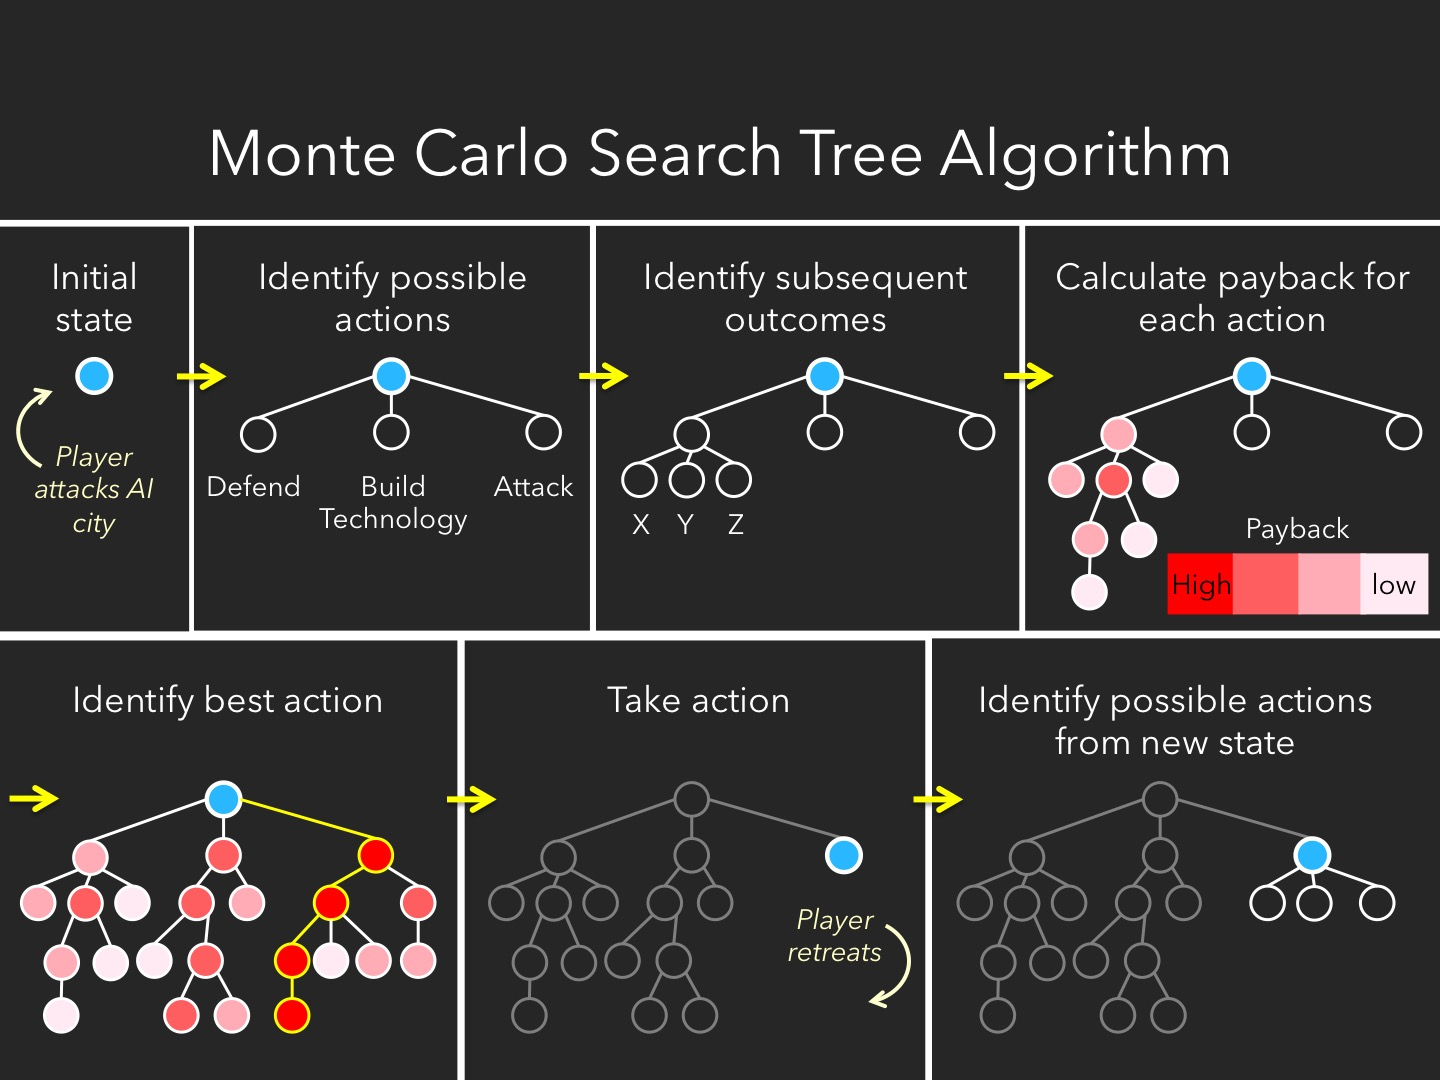
\includegraphics[width=\linewidth]{MCTS.jpg}
	\caption{Monte Carlo Tree Search \cite{lou2017}}
	\label{fig:mcts}
\end{figure}

\begin{figure}
	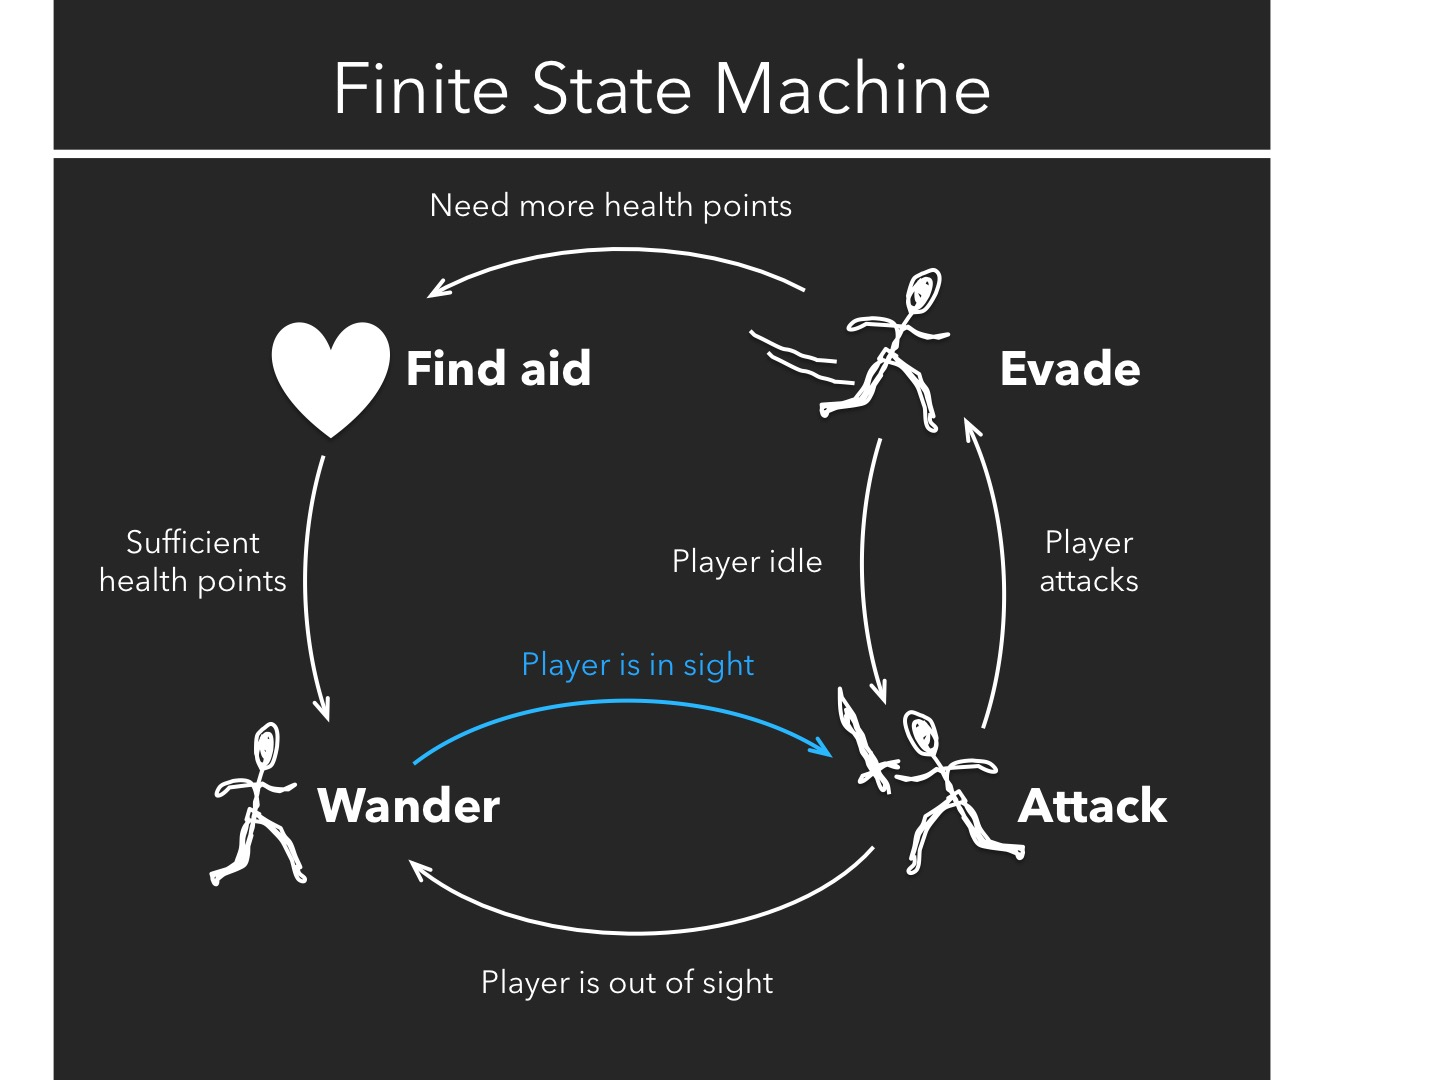
\includegraphics[width=\linewidth]{FSM.jpg}
	\caption{Finite State Machine \cite{lou2017}}
	\label{fig:fsm}
\end{figure}

\section{Related Work} %213
The main focus of this paper is to demonstrate a potentially valuable AI behaviour that is not complex yet efficient in enhancing smart AI. In section different AI implementation methods will be discussed, both complex and simple as well as why and how AI is used both in games and real life. This will include human curiosity and discuss it from a psychological view, why it's one of the main factors towards human's willingness to learn and gain new knowledge and some relevant learning algorithm implementations to make interesting and smart AI. Turing's Test will also be included in this section, which will describe it's use, advantages, and disadvantages and why it's used as a testing method for this project. Moreover, it will describe how smartness is going to be measured in this context. Methodology and hypotheses will be reviewed in sections III and IV respectively. The methodology will also include research artefact, introduce to what the participants will be asked to do and how data will be collected. The proposed behaviour implementation will be handled in Unreal Engine 4.22.3 using our team's game, which can be found in appendix \ref{appendix:a}, for easier testing purpose as there will be enough assets to create a unique world which AI could be tested on.

\subsection{AI Importance in Games} %382
Artificial intelligence has a big place in the modern world. Robots are being created to ease human life, machines that can beat the best players in the world in most complex games such as Go \cite{alphago} or chess. But AI for games is not created to overcome a player's abilities. It's there to enhance player's experience, to make the game more engaging and fun to play \cite{aiinvideogames} while acting realistically \cite{chaslot2008monte}. Therefore, other difficult problems are being solved, which may not fit well with AI used in real life, but they are still very valuable. Solving AI problems using games has become pretty common nowadays and is used for many areas as a testing purpose \cite{schaul2011measuring}. The testbeds can alter from simplicity to diversity \cite{schaul2011measuring} and can include testing natural language understanding and/or production, theorem proving, physical and simulated robotics and the original Turing's test \cite{schaul2011measuring}.

AI for games is mainly developed to increase a player's engagement and/or satisfaction feelings \cite{halo2}. Whether that's bosses or companions, friends or enemies. Given the flexibility of AI, games use it very differently. Thus, some games decide to enhance players' positive emotions and some might make the game feel terrifying. It is the designers' aspiration to create such feelings depending on the game itself. The satisfaction from hard challenges that required patience and dedication over many hours to practice to overcome, which makes them unforgettable as well as the fright from the ever building up atmosphere enhanced by terrifying creatures. All of this makes games unique and entertaining for people whose desire is to rest from our real world.

Of course, not every game must have AI, but what's the most frustrating a game can have is experience ruining AI. In which case, immersion breaks and players start complaining about the game being "unplayable" even though it's only enemies or friends behaving inappropriately or silly. Indeed, when players want to have a relaxing time playing a game, which is broken by AI only is upsetting. This again shows how important AI is for games, which requires a considerable amount of effort put into to create fun and engaging experience. So, to prove this point, the next couple of paragraphs will present and discuss the successful use of AI creating either positive or negative emotions in (1) Alien: Isolation and (2) Halo 2.

\begin{figure}
	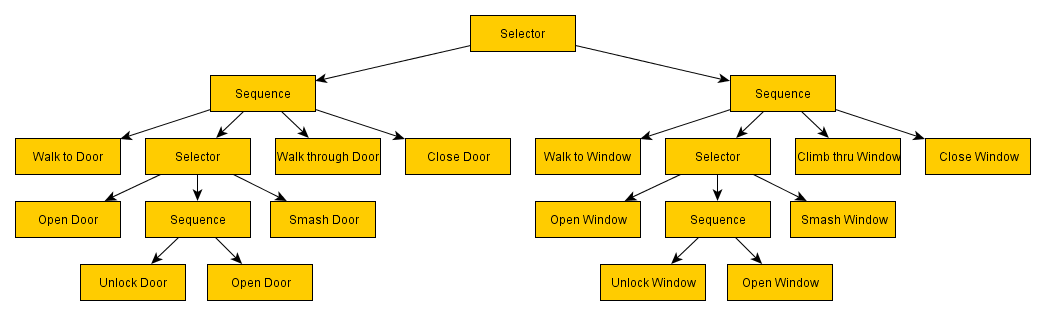
\includegraphics[width=\linewidth]{BehaviourTree.PNG}
	\caption{Behaviour Tree \cite{chris2014}}
	\label{fig:bt}
\end{figure}

\subsubsection{Alien: Isolation} %192
Artificial intelligence is very commonly used to create various feelings alongside an atmosphere of the game. A good example of this is a game called Alien: Isolation created by Creative Assembly, Feral Interactive and awarded a BAFTA Games Award for Audio Achievement. The alien enemy is the main threat that makes the player fear it to create a horrifying experience. However, the atmosphere around it accompanied by audio also plays a huge role. Moreover, specifically in this game, the AI is very complex and smart. In fact, it has two personalities, in other words - brains \cite{seller2019horrific}. The first one playing the role of the Alien ``having perfect information about the environment" \cite{seller2019horrific} and the second one responsible for movement and immediate stimuli response \cite{seller2019horrific}. Indeed, this together creates a very interesting and exceptional behaviour of the AI. The alien reacts to any sudden movements, noises and other characters that are not a player. In fact, there are other enemies besides aliens, which the alien itself attacks. This creates different scenarios and entertaining gameplay where a player can bait the alien to kill any hazard on the player's way that is another NPC.

\subsubsection{Halo 2} % 301
Another excellent example of smart and flexible AI in Halo 2 developed by Bungie Studios, which used the previously mentioned technique - behaviour trees \cite{behaviourtreeofhalo2}. AI in Halo 2 ``lives in a simulated world" \cite{halo2} - emphasizes Chris Butcher, one of four Engineering Leads at Bungie Studios, who was responsible for certain sections of Halo's development - and there's a very small distinction between NPCs and the player \cite{halo2}. Although every creature in Halo 2 feels unique they all function the same. NPCs perceive the world using their "senses", interpret all this data and make decisions based on them \cite{halo2}. This is mostly the same capabilities human players have. Therefore, this makes AI feel very smart, fun to play against and, more importantly, feel like a real human player. In addition, players can witness AI characters getting surprised, making mistakes and questionable decisions \cite{halo2} because they perceive their environment the same way a human player would. This particularly makes AI predictable, which was the aim of Halo 2 making NPCs consistent \cite{halo2} and is considered to be "smart" AI \cite{gamemakertoolkit}. Thus, players can predict NPCs' actions, but the consequences will be unpredictable.

Even more impressive feature AI in Halo 2 has is their joint behaviour system \cite{halo2}. It allows NPCs to communicate with each other and inform other allies of any threats or request a tactical move. This wouldn't be possible for players to notice if developers didn't add a speech to it. Indeed, whenever an enemy does any action, it is followed by it saying it out loud. This is a simple if/then statement, but it improves AIs predictability, which therefore increases its smartness as was mentioned before. In fact, small features that don't exactly relate to AI implementation might also enhance the way it feels, making it "smart" and unique.

\subsection{Curiosity} %478
Curiosity is a driving force for human exploration, which consists of exploration, investigation and learning behaviours \cite{wu2013curiosity}\cite{kashdan2004curiosity}. It makes people chase for knowledge and investigate anything new and potentially valuable. Moreover, curiosity is beneficial for people on two levels: the individual and the social \cite{kashdan2010curiosity}. The first one is represented as the "innate love of learning and of knowledge... without the lure of any profit" \cite{loewenstein1994psychology}. The social level, on the other hand, is presented as ``an ingredient for enhancing personal relationships'' \cite{wu2013curiosity}.

In computational form, curiosity can be split into different designs \cite{wu2013curiosity}. However, in this case, we are going to look at a curious exploratory agent. It can reach high learning effectiveness in an unknown environment \cite{wu2013curiosity}\cite{macedo2005role}. Even though the behaviour this project is going to test will be hard-coded, it gives opportunity for further learning, such as having a learning algorithm like curiosity-driven instead of hard-coding. Moreover, due to curiosity being proposed as algorithmic principles \cite{wu2013curiosity}\cite{pang2009curiosity}\cite{karaoguz2011curiosity} it enhances machines' "exploration" and allows it to own ``the desire to improve the model network's knowledge about the world." \cite{schmidhuber1991possibility}. It also had success in unsupervised developmental robotics \cite{schmidhuber2006developmental}\cite{oudeyer2004intelligent}.

Curiosity-driven learning in games can show some fascinating results. In \cite{burda2018large}, researchers train AI using curiosity-driven learning without extrinsic rewards and test it on dozens of games, 48 of which are Atari games. Previously, this kind of learning was using an either extrinsic or intrinsic reward system, however, this paper applies no rewards for AI and yet demonstrates positive results. The research has also been using Random Network Distillation (RND), which showed significant progress in \textit{Montezuma's Revenge} \cite{openairl}\cite{montezumarevenge}. It scored more than twice as high as an average human player, which shows potential in future development. However, this kind of learning doesn't always score as high as in \textit{Montezuma's Revenge}. This shows that it still requires improvements to be used in today's games and potentially in robotics.

The way curiosity-driven learning works is that the AI is given curiosity element into its learning and therefore it start to explore its environment. However, having only curiosity-driven learning is not always beneficial. (citation here) uses next-state prediction extension to improve curiosity-driven AI. The algorithm behind next-state prediction is that AI tries to predict what state of the game the AI will be in in the next frame. This kind of extension had success in exploring games and eventually getting higher scores than human players. However, there's one problem researchers stumble upon - noisy-TV problem. In fact, it totally break the AI while the algorithm is still working as intented. The meaning behind it is when the AI sees a random sequence of images in front of it, it tries to predict what the next image will be, therefore, getting stuck watching it. Thus, it is called noisy-TV problem, due to old TVs black and white screen noise it has when not working.

\subsection{Turing's Test}
``I believe that in about fifty years it will be possible to program computers... to make them play the imitation game so well that an average interrogator will not have more than 70 per cent chance of making the right identification after five minutes of questioning" \cite{alan59turing}. These are the words of Alan Turing, who inspired the creation of machine learning \cite{hayes1995turing}. He created an imitation game, which is a testing game that considers whether a machine can think \cite{alan59turing}. The way it originally works is an interrogator, that stays apart from the other two people that are a different gender, questions these two subjects. The goal of the interrogator is to identify which of the two is the man and which is the woman \cite{alan59turing}. However, there are different interpretations of this game. Specifically for AI testing, one of the subjects is a machine and the other is human. A computer terminal is used in this case to question subjects \cite{livingstone2006turing}. %167

However, this has been criticized in many ways \cite{hayes1995turing}\cite{sweeney2003s}\cite{crockett1994turing}\cite{livingstone2006turing}. In fact, some consider, that researchers are trying to only pass this test no matter what, thus excluding the important details of their implementation \cite{hayes1995turing}. It has become a standard for AI these days and therefore researchers tend to lean towards confirming the null hypothesis \cite{hayes1995turing}. Another issue proposed in \cite{hayes1995turing} is that it is not always clear what the study is trying to detect. It has to be clear at all times what is being measured and what exactly that measurement represents. %92

Even though Turing's test is being criticised very broadly, this project is still going to use this kind of test. However, it will not be identical to the original one nor be similar to the imitation game. In fact, there will be no subjects and only an interrogator. Therefore, the interrogator, or in other words, participant, will not be able to ask questions, but only view the AI and human behaviours and try to distinguish them. Thus, most of the criticism presented in \cite{hayes1995turing}\cite{sweeney2003s}\cite{crockett1994turing}\cite{livingstone2006turing} will not be mitigated. So, how will this paper measure proposed "smartness" of AI? Practically, there are no certain measurements for intelligence thereby researchers make up their own measurements for AI depending on their study. Though one statement sums up all the aspects of intelligent agents pretty clearly - ``Intelligence is a very general mental capability that, among other things, involves the ability to reason, plan, solve problems, think abstractly, comprehend complex ideas, learn quickly and learn from experience." \cite{gottfredson1997mainstream}. Paper \cite{legg2007universal} proposes measures for an intelligent agent to be the ``ability to achieve goals in a wide range of environments.". As this project is looking particularly into exploration extension for AI behaviour, this statement becomes appropriate. %202

\section{Hypotheses}
The aim of this project is to implement a simple exploration extension for AI behaviour based on human's curiosity. Therefore, this project's first hypothesis is that exploration extension will perceive AI smartness compared to non-curious AI. The second hypothesis aims the participants to distinguish the player's behaviour from AI's behaviour, which will be provided by the questionnaire data. After analysing this data, the results will show whether the curious behaviour is leaning towards human-like, which will prove or disprove this project's hypothesis.%82

[Put a hypotheses table here after I change the wording]

These hypotheses are mainly aimed to see if exploration behaviour based on human's curiosity enhances smartness for AI in games. Due to AI in games primarily being used for NPCs and concentrated on combat systems, idle states are often excluded from having "smart" behaviour. This is done in order to save the computer's resources for a more important matter, such as combat. However, having a smart looking AI for walking simulators can, therefore, enhance a player's experience in such genres. This could become a decisive factor for developers that want to create a gorgeous walking simulator using a fantastic looking environment enhanced with smart and interesting artificial intelligence. %108

\section{Methodology}
\begin{table}
	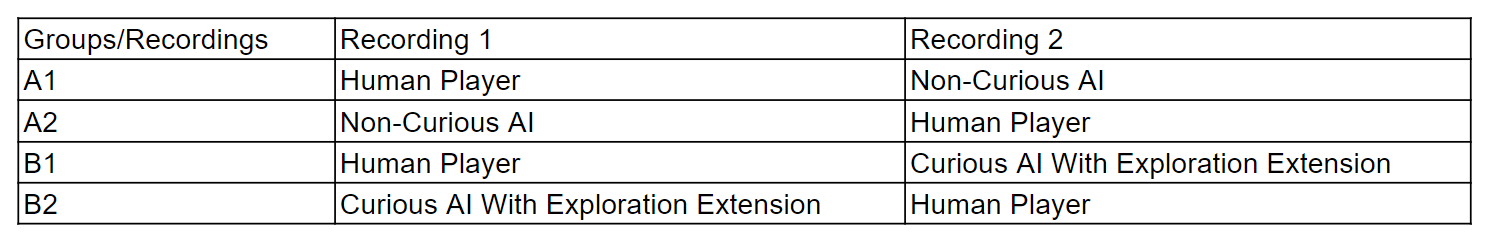
\includegraphics[width=\linewidth]{MethodologyTable.PNG}
	\caption{Methodology}
	\label{tab:methodology}
\end{table}
The testing of the hypotheses will be handled by separating participants into four groups, two main groups and two sub-groups, randomly chosen and shown video recordings selected at random using random number generator, see Table \ref{tab:methodology}. The first group will be presented with non-curious AI behaviour and the human player's behaviour or vice versa. The second group, on the other hand, will be introduced with curious AI behaviour, which was enhanced by exploration extension, and human player's behaviour or vice versa. All of this will be done randomly to minimise bias towards either side as much as possible. %89

\subsection{Research Artefact} %171
For the proposed hypotheses testing the project will be using our team project game that is made using Unreal Engine 4 with a few changes in the game to represent first-person walking simulator and can be found in appendix \ref{appendix:a}. The environment in the game will also be changed in order to more accurately generate curiosity from both AI and player perspectives. Moreover, the exploration behaviour this paper is going to test will be implemented using Behaviour Tree. The behaviour will be thoroughly tested for any ` experience ruining errors and pilot-tested before the start of the research. Afterward, it will be recorded and, during the testing process, data will be gathered from participants. Another AI behaviour will also be recorded before the data gathering as well as human's behaviour. Both AI behaviours will have the same base and only one will be enhanced by exploration. Also, all the recordings will be handled by the free recording software called Open Broadcaster Software (OBS) due to its simplicity and quality of entries.

\begin{figure}
	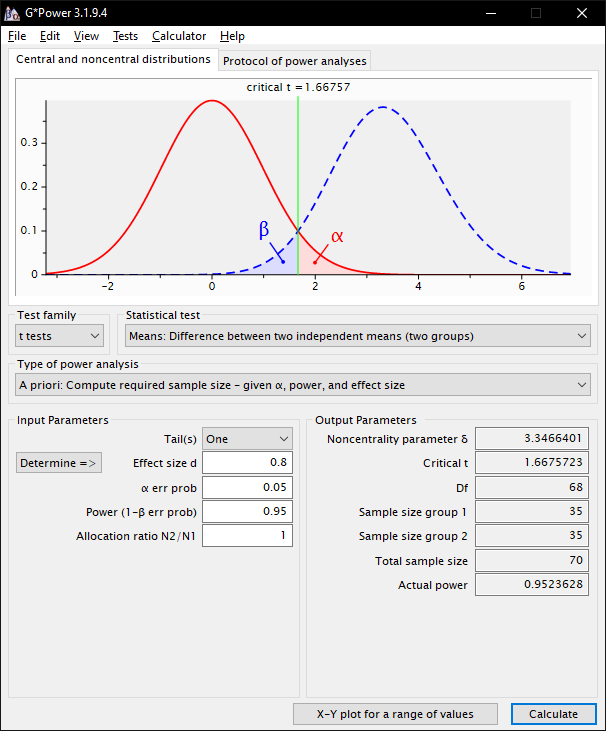
\includegraphics[width=\linewidth]{GPower.PNG}
	\caption{Screenshot of a-priori power analysis to calculate sample size using G*Power available at: http://www.gpower.hhu.de/}
	\label{fig:gpower}
\end{figure}

\subsection{Participants} %201
Due to the need for a human player's behaviour, seven to eight people will be asked to play the game and record their gameplay. This necessity does not require a lot of participants and, moreover, they will not be taking part in providing research data and are not counted towards the required sample size presented in Figure \ref{fig:gpower}. Ideally, they will have no to little experience with such games to generate a more curious nature of humans. The goal for these participants will be to explore the game's environment. However, they will not be told so to avoid bias towards having unnatural curiosity behaviour, which could influence the project's testing. Instead, they will have the ability to do whatever they desire. This will instead generate more natural behaviour and thought processes from these participants and will benefit this project's outcome. It will be handled in the first place before collecting the necessary data to analyse later in the paper. Player recordings will also help with AI development as they give an ability to observe player behaviours that could potentially be implementated for AI to imitate human-like actions.

The participants that are going to take part in the research and answer the questionnaire will likely be from different disciplines both inside and outside of Falmouth University's Games Academy due to bigger audience variety and experience in such field. There will be two groups of participants, each group being divided into another two sub-groups (see Table \ref{tab:methodology}), observing different recordings of human player and AI behaviours that are selected randomly as shown in Figure \ref{fig:gpower}. The study will require a minimum of 70 participants, 35 of each main group, given the effect size of 0.8, which is considered large by Cohen's guidelines \cite{cohen1992power}. However, if the project brings more attention, the sample size could be increased accordingly, giving more data to analyse and potentially have sufficient results. %149

\subsection{Questionnaire} \label{data} %204
After the participants have viewed the recordings, they will be asked to complete a survey. The survey will provide the necessary data to analyse and later discuss the efficiency of the proposed exploration behaviour enhancing the AI's smartness. First of all, the survey will ask how often the participant plays games and whether they have played any first-person walking simulators. This will give an understanding of the participant's experience with games, which might influence their insight into the research. The second part of this survey consists only of one question asking which behaviour felt smarter in their opinion before getting the necessary data to analyse curiosity in each behaviour. The last part consists of measuring behaviours' curiosity level using a scale from one to seven and asking the participants whether they have distinguished an AI from human. In which case, if the answer to this question is positive, they will be asked to answer two more questions that include a short description of the distinguishable features AI had and how smart it felt on a scale of one to seven. This will give more detailed data to analyse regarding AI. Furthermore, the sample code for analysing this data can be found in the appendix \ref{appendix:b}

\subsection{Data Management Plan}
[Add tables of questions]
[Talk about why specifically these questions, how am I going to interpret it]

\subsection{Ethics}
Ethics had to be concerned due to the Falmouth Research Ethics Policy. For both parts of data collection no personal data was collected that could identify a specific participant. Hence, the data is considered low-risk. However, having two parts of data collection, two different consent forms and informations sheets had to be written depending on the data collected during that part. Information sheets had to be writted to give participants' a brief idea of what the research study is about. It also states that the participation is entirely voluntary and could be withdrawn at any time without giving any reason. These can be seen in the study's repository [add footnote to dissertation repo here].

For the first part of data collection a consent form stating that participant's gameplay will be recorded had to be mentioned. Thus, a different consent form requesting their agreement of participation had to be made. However, as mentioned before, this part still has low-risk for personally-identifiable data, as nothing except for game screen was recorded. These participant were also asked to answer a few questions after playing, which were not necessary, but potentially valuable to improve or imitate player actions for AI as well as used in analysis. This is further discussed in Section \ref{data}.

Second part of data collection would also require these papers, however, there's still no personal data required. The only questions that were asked to answer are mentioned in Section \ref{data}. This data is also stored anonymously, same as the previously mentioned one, and will be retained for approximately 6-month period. Afterwards, all data will be deleted to prevent any information leakage outside this study anytime.

Regarding game demo there are no legal, social or professional concerns. The demo is made exceptionally to test AI, where environment to observe is vivid and reach, and doesn't serve any purpose for human player gameplay. The assets used in the demo are free and were downloaded from Unreal Engine Marketplace [add footnote here???] and are credited in the text file in the research artefact's repository [add footnote to artefact repo here].

%These participants will be asked to given an information sheet in the survey itself to understand the purpose of this study and what they are asked to do as well as being able to withdraw at any time. In addition, a consent form will be provided to sign, saying that their participation is voluntary, before starting the study. 

\section{Computing Artefact}
\subsection{Introduction}


\subsection{AI Behaviours}


\subsection{Life Cycle}
\cite{isaias2015information}
For this research artefact a combination of V-model and star-model have been chosen. This is done with the fact that one is more structured regarding design, implementation and testing. However it lacks freedom of choice in terms of task allocation. It was beneficial for the artefact to allow more flexibility in development due to variety of behaviour required and some features for both AI and player to grant for better imitation of game exploration. However, consistent testing was required to verify that all the important features are working as well as AI behaviour are acting as expected, which V-model allows very well. If any of the features or behaviours break during the development process, an act of redesigning or reworking ir required.
A story board was being updated throughout the development whenever a task was in progress, completed or a new one added. In addition to that, notes have been taken during the development process to track current bugs and to-do tasks at the time.

\subsection{Testing}
Artefact testing was handled regularly to ensure that the most important AI features were being functional. In order to keep track of these tests, a test plan was written beforehand to provide the necessary tests for the project. The test plan was written with a step-by-step guide of how a particular function will be tested as well as updated whenever the test was first handled. These tests were managed by two different methods: 
\begin{itemize}
	\item Unreal Engine's built-in plugin - Automation system
	\item Unit test
	\item Observing??
\end{itemize}
Automation system is a system that automatically tests any features and/or functions if an appropriate code has been written. It drastically decreases the time of discovering bugs, which keeps the software with as fewer problems as possible. Due to complexity of keeping AI fully functional, such systems are very beneficial for both small and big projects. It had greatly helped detect any crucial issues regarding AI, especially having limited time for the development.
How was unit tests handled? were they even done?
Testing by observing. Is it valuable?

\section{Results}
\subsection{AI Improvements}

\subsection{Player Behaviour}

\section{Discussion}

\section{Conclusion} %92
So, in conclusion, artificial intelligence for games is very important in today's games, however, terminology "smart" is interpreted differently. It is not about winning human player's all the time how it is to maintain the game's fun and satisfaction levels. Moreover, games are also used as testbeds for AI, which can further improve real-life robotics. Robots, however, are becoming more and more advanced hence making curiosity for robots more feasible. Even though curiosity is becoming more possible for robots there are still other major problems to be solved before it becomes real.

% references section

\bibliographystyle{IEEEtran}
\bibliography{References}

% Appendices

\appendices
\section{First appendix}
\label{appendix:a}
As mentioned in the paper, project's computing artefact will be based of team's project game. The repository for that is gamesgit.falmouth.ac.uk/users/tm200066/repos/computing-artefact/browse and the only part that will be modified for the computing artefact is located in Content/Artificial\_Intelligence. However, some unrelated to AI aspects will potentially be added, such as assets from other team members, to change the environment the AI is going to be placed in.

\newpage

\section{Second appendix}
\label{appendix:b}
\begin{lstlisting}[frame=single, breaklines=true][language=R]
	# Install the necessary packages
	install.packages("readr")

	library("readr")

	# Import a CSV file and save it to a variable
	data <- read.csv("C:/3Year/Dissertation/Research Test/ResearchTest.csv")

	# Assign variables to question results for easier readability and usability
	Player <- data$How.curious.did.the.player.feel.about.the.environment.
	AI <- data$How.curious.did.the.AI.feel.about.the.environment..

	# Use one-tailed t-test to calculate difference between means that also gives p-value
	t.test(Player, AI, paired = TRUE, alternative = "greater")
\end{lstlisting}

\section{Testing}
Put any testing screenshots and test plan here.

\section{Self-Reflection}
Some introduction here - I hate my life and all that

\subsection{Dispositional} %230
Keeping motivation for the dissertation writing was hard due to the high enjoyment of the team game project. Throughout this academic year, I have been enjoying our team game project development. Team composition and relationship between each other have been positive from the very beginning. Therefore, I was dedicating all my time to our team and the game. Thus, keeping my motivation for the dissertation project was much less than game development. So, I was behind the schedule and my peers, which made me nervous that I will struggle a lot later. Eventually, it happened and I had to make myself concentrate entirely on the dissertation putting the game aside, which resulted in me constantly trying to keep motivation for work. Moreover, a world pandemic happened and everyone was forced to work from home, which made it even harder to inspire me to work. This could've potentially been avoided if only I have had a dedicated schedule for both my projects. A framework of at least a half an hour of work doing dissertation writing or artefact would've changed a lot. I would still be working on the game most of my time, however, with this structure, I could've been doing progress on my dissertation constantly. This would have made things much easier later on and grown a habit of having a dedicated schedule for working hours.

\subsection{Cognitive}
Write about my understanding of AI implementation in Unreal?????

\subsection{Affective}
Stress and frustration from just thinking about the deadline that's very quickly approaching.

\subsection{Procedural}
AI is prone to break a lot so debugging skills for such area is very useful???

\subsection{Interpersonal}
Supervisor meetings have helped greatly in keeping my head up as well as some pieces of advice from my peers. However, I felt like I had less help from these meetings due to my anxiety of asking for advice and thinking everything's alright.

\subsection{Conclusion}

% Unused
% This is essential because of the nature of some recordings to be likely of not providing the necessary curiosity for more accurate testing purpose (participants)
% Explain curiosity - human behaviour often depends on person's intentions to explore. Why apply to AI? The aim of this paper is not to create curiosity-driven AI in Unreal Engine 4 (UE4), but to implement and test a particular behaviour and see how people react. Whether they like it or not, whether they think it behaves smart and etc. The aim of this implementation is to find a small nuance that can make the AI feel and act smarter.
% Statechart-Based AI in Practice
% Monte-Carlo Tree Search: A New Framework for Game AI
% Building Human-Level AI for Real-Time Strategy Games

% that's all folks
\end{document}
